\documentclass[11pt,oneside,a4paper,final]{article}
\usepackage{geometry}                % See geometry.pdf to learn the layout options. There are lots.
\geometry{a4paper}                   % ... or a4paper or a5paper or ... 
%\geometry{landscape}                % Activate for for rotated page geometry
%\usepackage[parfill]{parskip}    % Activate to begin paragraphs with an empty line rather than an indent
\usepackage{graphicx}
\usepackage[caption=false,font=footnotesize]{subfig}
\usepackage{epstopdf}
\usepackage{url}
\usepackage[hidelinks]{hyperref}

\usepackage[british=nohyphenation]{hyphsubst}
\usepackage[british]{babel}
\usepackage[T1]{fontenc}
\usepackage{times}

\title{Assignment (20\%)}
\author{ICP3029 / ICP4127}
\date{Deadline: 11th April 2014}                                           % Activate to display a given date or no date

\begin{document}
\maketitle
%\section{}
%\subsection{}

\sloppy

The assignment is due at midnight on Friday 11th April. 
Submissions must be made via Blackboard. 
Please take into account upload times and internet connections when considering how much time you have remaining. 
Late submissions will be dealt with in accordance with University policy. \\

%This assignment is designed to test your ability to grasp information, and to reflect upon it in relation to what you have already learnt.\\

The assignment is based on a set of functions to build 3D implicit surfaces. 
These represent contours (or isosurfaces) through a scalar field in 3D. 
It is a relatively common methods for creating smooth 3D surfaces. 
Figure~\ref{fig:2D slices} shows slices of such a scalar field. 
It is built using 3~control points. 
%
Figure~\ref{fig:3D rendering} isosurfaces of the same scalar field. 
They are extracted using the Marching-cubes algorithm with different threshold values. 
\begin{figure}[tb]
	\centering
	\subfloat[150\textsuperscript{th} slice.]{
\includegraphics[width=0.2\linewidth]{slide_150.png}}\quad
	\subfloat[220\textsuperscript{th} slice.]{
\includegraphics[width=0.2\linewidth]{slide_220.png}}\quad
	\subfloat[300\textsuperscript{th} slice.]{
\includegraphics[width=0.2\linewidth]{slide_300.png}}\quad
	\subfloat[340\textsuperscript{th} slice.]{
\includegraphics[width=0.2\linewidth]{slide_340.png}}

 \caption{\label{fig:2D slices} Slices of a scalar field build using 3~control points with the \emph{Meta Balls} density function.}
\end{figure}
\begin{figure}[tb]
	\centering
	\subfloat[Threshold: 0.0125.]{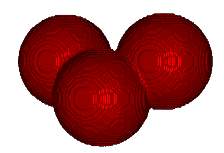
\includegraphics[width=0.2\linewidth]{threshold_00125.png}}\quad
	\subfloat[Threshold: 0.125.]{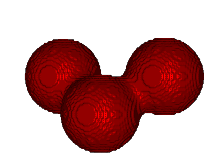
\includegraphics[width=0.2\linewidth]{threshold_0125.png}}\quad
	\subfloat[Threshold: 0.25.]{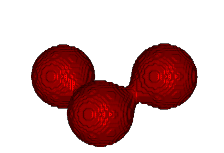
\includegraphics[width=0.2\linewidth]{threshold_025.png}}\quad
	\subfloat[Threshold: 0.5.]{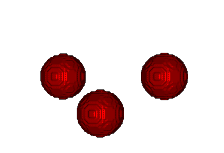
\includegraphics[width=0.2\linewidth]{threshold_05.png}}
	
 \caption{\label{fig:3D rendering} Isosurfaces extracted from the volume presented in Figure~\ref{fig:2D slices} using marching cubes with different threshold values.}
\end{figure}

It is not required to know what implicit surfaces are to complete this assignment. 
To know more about implicit surfaces, a good tutorial is available at:
\url{http://paulbourke.net/geometry/implicitsurf/}.

To extract and build the code that is provided -- after having set the development environment on HPC Wales -- proceed as follows:
\begin{footnotesize}
\begin{verbatim}
 $ tar zxvfp MPI_assignment.tar.gz  # Decompress the archive
 $ cd MPI_assignment                # Go to the assignment directory
 $ ls                               # See the content of the directory
 $ cd build                         # Go to the build directory
 $ make                             # Build the project
 $ ./test                           # Run the test program
\end{verbatim}
\end{footnotesize}
When you run the test program, a volume data set will be created. 
It contains $512 \times 512 \times 512$ voxels stored sequentially using floating-point numbers with single precision (i.e.~32~bits).
To view the content of the file, you may use ImageJ on your standard PC/laptop at home or in the lab.

We provide the initial working -- but inefficient -- C++ program (it is not parallelised). 
The assignment is to make this more efficient (as described in class) using parallel processing with MPI, and provide
evidence of such by timing both the original and improved version. 
Experiments should include:
\begin{itemize}
\item Using various numbers of control points,
\item Using various numbers of processors, and 
\item Comparing the performance using the GNU (g++) and Intel (icc) compilers.
\end{itemize}

Your final submissions should include the code and a report that discusses the changes you made to the program and the experiments showing performance. 
You should discuss for what problems sizes parallelisation is effective. 
You should submit results showing speed-up curves. 
The initial inefficient code is in the file \verb!src/ImplicitSurface.cxx! in the function \verb!void voxelise(...)!. 
%and a gnuplot script to plot results is in \verb!plot/plotpart.plt!.

\vfill
\end{document}  